\documentclass[aspectratio=169]{beamer}
\beamertemplatenavigationsymbolsempty
\setbeamercolor{frametitle}{fg=black}
\usepackage{amsmath,xcolor,enumitem}
\usepackage{algorithm,siunitx}
\usepackage[noend]{algorithmic}
\setbeamertemplate{frametitle}[default][center]
\usepackage{booktabs}
\usepackage{hyperref}
\usepackage{subcaption}
\usepackage{media9}

\usepackage{tikz}
\usetikzlibrary{shapes, arrows.meta, positioning, arrows}


\title{Design optimization of compliant mechanisms\\
\large ME46115 Compliant Mechanisms (2022/23 Q1)}
\author{by Stijn Koppen\\
with thanks to Dirk Munro, Davood Machekposhti, Matthijs Langelaar, and you}
\date{16 November 2022}

\begin{document}
\maketitle

% \begin{frame}
%     \centering
%     \includegraphics[height=0.8\textheight]{fig/rotflex.png}
% \end{frame}

% \begin{frame} 
% \begin{center}
% \includemedia[
%     activate=onclick,
%     width=0.75\textwidth
% ]{\includegraphics{fig/rotflex.png}}{movies/defmirror.mp4}
% \end{center}
% \end{frame}

% \begin{frame}

% % \begin{center}
% % \begin{description}
% % \item[2015] Bachelor of Engineering (BEng) at HHS
% % \item[2018] Master of Science (MSc) at TUD-PME
% % \item[2022] Doctor of Philosophy (PhD) at TUD-PME
% % \item[2024] Postdoc at TUD-PME
% % \end{description}
% % \end{center}

% \end{frame}

\begin{frame}{goals and outline}

% you will learn why and when (not) to use optimization as a design tool
% you will learn how to convert a design problem to an optimization problem formulation
% you will learn how to choose a fitting algorithm to solve your problem
% you will learn about the most important considerations in design optimization based
% you will learn the basics of sensitivity analysis

% disclaimers:
% you will not become an optimization expert (take optimization course)
% you will not have a working optimization routine, but you will know how to build your own!

\centering
\begin{minipage}[c]{.8\textwidth}
at the end of this lecture you can

\begin{itemize}[itemsep=1.5em]
\pause
    \item[\checkmark] understand optimization problem formulations \pause
    \item[\checkmark] translate your design problem to an optimization problem \pause
    \item[\checkmark] understand the model-based iterative optimization process \pause
    \item[\checkmark] choose an optimization that fits your optimization problem\pause 
    \item[\checkmark] know a bit about sensitivity analysis
    \pause
    \item[\checkmark] value optimization for compliant mechanism design
\end{itemize}
\end{minipage}
\vfill
\centering
% course material: \href{http://www.github.com/artofscience/me46115}{github.com/artofscience/me46115}

\end{frame}

\begin{frame}{design optimization: when and why?}

% improve performance of existing design
% improve robustness

% find best solution (i) within given time, or (ii) least function eval

\centering
\begin{minipage}[c]{.7\textwidth}
\begin{itemize}[itemsep=1.5em]
\pause
\item[\checkmark] concept generation (topology optimization)
\pause
\item[\checkmark] improve performance of existing design
\pause
\item[\checkmark] provides insight in design problem
\pause
\item[\checkmark] systematic approach to problem solving (speedup and performance)
\end{itemize}
\end{minipage}
\end{frame}


% \begin{frame}{curse of dimensionality}

% % why not try all options and pick the best?

% % say we have n variables and for each variable we check s options, then this would require s^n model evaluations

% % say 10 variables, and 10 samples per variable and model evaluation just takes 1s, then this will take 317 years!

% \begin{center}
% why not brute-force the problem?
% \end{center}

% \begin{center}
% \begin{equation*}
% \left.
%     \begin{aligned}
%     n \quad &\text{variables}\\
%     s \quad &\text{samples per variable}\\
%     \end{aligned} ~ \right\}
%     \quad s^n \quad \text{model evaluations}
% \end{equation*}

% % \begin{equation*}
% % \left.
% %     \begin{aligned}
% %     \SI{100}{} \quad &\text{variables}\\
% %     \SI{2}{} \quad &\text{samples per variable}\\
% %     \SI{1}{\second} \quad &\text{time per evaluation}
% %     \end{aligned} ~ \right\}
% %     \quad 1 \cdot 2^{100} =  \SI{1}{} ~ \text{years}
% % \end{equation*}
% \end{center}

% \end{frame}



\begin{frame}{optimization problem formulation}

% optimizatiaon problem P: find the/an solution of design/decision/optimization variables x that minimizes g0 whilst satisfying constraints gi within design space X.
% n design variables
% m constraints

% note: max x = min -x or min 1/x
% note hi[x] = bh can be written as two inequality constraints!

\vfill

\begin{columns}
\begin{column}{.5\textwidth}
\centering
\begin{align*}
\begin{aligned}
\underset{\mathbf{x}}{\text{minimize}}  &&& f\left[\mathbf{x}\right]\\
\text{subject to} &&& \mathbf{g}\left[\mathbf{x}\right] \leq \bar{\mathbf{g}}\\
&&& \underline{\mathbf{x}} \leq \mathbf{x} \leq \overline{\mathbf{x}}
\end{aligned}
\end{align*}
\end{column}

\begin{column}{.6\textwidth}
\centering
\begin{itemize}
\pause
    \item unconstrained vs. \underline{constrained} problem
    \item \underline{continuous} vs. discrete variables
    \pause
    \item \underline{differentiable} vs. non-differentiable functions
    \pause
    \item unimodal vs. \underline{multimodal} problem
\end{itemize}
\end{column}

\end{columns}

\vfill

\centering
\pause
typically no closed-form solution

% \begin{minipage}[c]{\textwidth}
% \begin{description}
%     \item[$\mathcal{P}$] optimization problem
%     \item[$\mathbf{x} \subseteq \mathcal{R}^n$] design variables
%     \item[$\underline{\mathbf{x}}$, $\overline{\mathbf{x}} \in \mathcal{R}^n$] variable bounds
%     \item[$\mathbf{x}^* \in \mathcal{R}^n$] solution
%     \item[${g_0\left[\mathbf{x}\right]} \in \mathcal{R}$] objective function
%     \item[${g_i\left[\mathbf{x}\right]} \in \mathcal{R}$] constraint function $i$
%     \item[${\bar{g_i}} \in \mathcal{R}$] max constraint value $i$
% \end{description}
% \end{minipage}

\end{frame}


\begin{frame}{optimization strategies}

% derivative-free, also called zeroth order, gradient-free
% gradient-based, subdivided in first-order and second-order approaches

% output for gradient-based also Lagrange multipliers; this tells something about how "active" the constraints are. 


\centering

\begin{table}
\begin{tabular}{r | p{2.5cm} | p{3.5cm}}
  &derivative-free & gradient-based \\
  \midrule
  inputs & $\mathbf{x}, f, \mathbf{g}$  &  $\mathbf{x}, f, \mathbf{g}, \frac{\text{d} f}{\text{d} \mathbf{x}}, \frac{\text{d} \mathbf{g}}{\text{d} \mathbf{x}}\color{gray},\frac{\text{d}^2 f}{\text{d} \mathbf{x}^2}, \frac{\text{d}^2 \mathbf{g}}{\text{d} \mathbf{x}^2}$\color{black} \\ 
  search space & global & \textcolor{red}{local} \\
  derivatives needed & no & \textcolor{red}{yes} \\
  efficiency & \textcolor{red}{low} & high \\
  number of variables & \textcolor{red}{low} & high \\
  implementation effort & low & \textcolor{red}{high}\\
  % examples & brute-force \newline direct search \newline stochastic \newline population-based \newline Bayesian \newline \ldots & line search \newline steepest descent \newline (quasi)-Newton method \newline SLP/SQP \newline interior point methods \newline \ldots \\
\end{tabular}
\end{table}

\end{frame}


\begin{frame}{model-based iterative optimization process}

% Model contains: system or state variables (g[u[x]]), system parameters or decision variables (h,b,L) and system constants e.g. E, rho.

% Make example of a model, e.g. flexure hinge.

% Every optimization routine has an initial guess, even if its random

% Termination / Convergence criteria

% The model may include a call to a FEA routine (e.g. ansys or own written)

% dg and d2gdx2 optional (only for gradient-based optimization)

% Optimization is about efficient use of information
% The more expensive the model is, the more important is efficient use of information
% Without providing the optimizer with information about the problem, the optimizer cannot be efficient

% Total cost (flops or time) ~ design iterations x model evaluations per iteration


\vfill
\begin{columns}
\begin{column}{.5\textwidth}
\centering
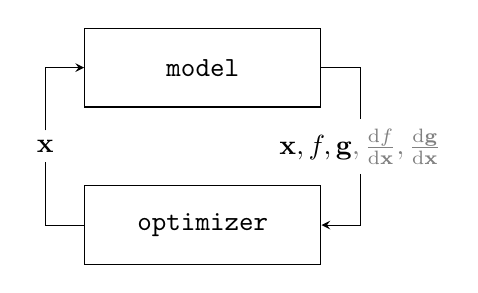
\begin{tikzpicture}
    \node[draw=none] at (2,0) (data) {$\mathbf{x}, f,\mathbf{g}\color{gray}, \frac{\text{d} f}{\text{d} \mathbf{x}},\frac{\text{d} \mathbf{g}}{\text{d} \mathbf{x}} \color{black}$};
    \node[draw=none] at (-2,0) (variables) {$\mathbf{x}$};
    \node[draw,
        minimum width=3cm,
        minimum height=1cm] at (0,1) (model) {\texttt{model}};
    \node[draw,
        minimum width=3cm, 
        minimum height=1cm] at (0,-1) (optimizer) {\texttt{optimizer}};
    \tikzstyle{connector} = [draw, -stealth];
    \tikzstyle{conn} = [draw, -]
    \path [conn] (model) -| (data);
    \path[connector] (data) |- (optimizer);
    \path[conn] (optimizer) -| (variables);
    \path[connector] (variables) |- (model);
\end{tikzpicture}
\end{column}
\begin{column}{.5\textwidth}
\centering
\begin{algorithmic}
\STATE $\mathbf{x} = \mathbf{x}_0$ 
% \WHILE{$c\left[\mathbf{x}, \mathbf{g} \color{gray}, \frac{\text{d} \mathbf{g}}{\text{d} \mathbf{x}},\frac{\text{d}^2\mathbf{g}}{\text{d} \mathbf{x}^2} \color{black} \right] > \epsilon$}
\WHILE{\text{not converged}}
\STATE $f, \mathbf{g}\color{gray}, \frac{\text{d} f}{\text{d} \mathbf{x}},\frac{\text{d} \mathbf{g}}{\text{d} \mathbf{x}} \color{black} = \texttt{model}\left[\mathbf{x}\right]$
\STATE $\mathbf{x} = \texttt{optimizer}\left[\mathbf{x}, f, \mathbf{g}\color{gray},\frac{\text{d} f}{\text{d} \mathbf{x}},\frac{\text{d} \mathbf{g}}{\text{d} \mathbf{x}} \color{black}\right]$
\ENDWHILE
\end{algorithmic}
\end{column}
\end{columns}
\vfill
\centering
\pause
\begin{equation*}
\text{computational effort} \approx \text{no. design iter} \times \text{no. model evaluations per iter} 
\end{equation*}

\end{frame}


\begin{frame}
\begin{center}
\vfill
\includegraphics[height=0.8\textheight]{fig/kk20121}
\quad \quad \quad 
\pause
\includegraphics[height=0.6\textheight]{fig/kk20122}
\end{center}

\footnotetext{\tiny Krishnan, Kim and Kota (2012) ``A metric to evaluate and synthesize distributed compliant mechanisms" in: Journal of Mechanical Design}    

\end{frame}

\begin{frame}
\begin{center}
    \includegraphics[height=0.7\textheight]{fig/kk20123}
    \quad \quad \quad
    \pause
    \includegraphics[height=0.7\textheight]{fig/kk20124}
\end{center}

\footnotetext{\tiny Krishnan, Kim and Kota (2012) ``A metric to evaluate and synthesize distributed compliant mechanisms" in: Journal of Mechanical Design}    

\end{frame}

\begin{frame}

\begin{center}
 \includegraphics[height=0.8\textheight]{fig/kk20126}
 \quad \quad \quad 
 \pause
 \includegraphics[height=0.7\textheight]{fig/kk20125}
\end{center}


\footnotetext{\tiny Krishnan, Kim and Kota (2012) ``A metric to evaluate and synthesize distributed compliant mechanisms" in: Journal of Mechanical Design}    

\end{frame}


\begin{frame}
\begin{center}
\includegraphics[height=0.65\textheight]{fig/kota20011}
\quad \quad \quad
\pause
\includegraphics[height=0.65\textheight]{fig/kota20012}
\quad \quad \quad
\pause
\includegraphics[height=0.65\textheight]{fig/kota20013}

\end{center}

\footnotetext{\tiny Kota, Joo, Li, Rodgers and Sniegowski (2001) ``Design of compliant mechanisms: applications to MEMS" in: Analog integrated circuits and signal processing}    

\end{frame}




\begin{frame}
\centering

\begin{columns}
\begin{column}{0.3\linewidth}
\begin{figure}
\begin{subfigure}{.4\textheight}
\centering
\includegraphics[width=\linewidth]{fig/lk2009domain}
\end{subfigure}
% \begin{subfigure}{.3\textheight}
% \centering
% \includegraphics[width=\linewidth]{fig/lk20091}
% \end{subfigure}
\pause
\begin{subfigure}{.4\textheight}
\centering
\includegraphics[width=\linewidth]{fig/lk20092}
\end{subfigure}
% \begin{subfigure}{.3\textheight}
% \centering
% \includegraphics[width=\linewidth]{fig/lk20093}
% \end{subfigure}
% \begin{subfigure}{.3\textheight}
% \centering
% \includegraphics[width=\linewidth]{fig/lk20094}
% \end{subfigure}
% \begin{subfigure}{.3\textheight}
% \centering
% \includegraphics[width=\linewidth]{fig/lk20098}
% \end{subfigure}
\end{figure}
\end{column}

\pause
\begin{column}{0.3\linewidth}
    \begin{figure}
\begin{subfigure}{.4\textheight}
\centering
\includegraphics[width=\linewidth]{fig/lk20095}
\end{subfigure}
\begin{subfigure}{.4\textheight}
\centering
\includegraphics[width=\linewidth]{fig/lk20096}
\end{subfigure}
% \begin{subfigure}{.3\textheight}
% \centering
% \includegraphics[width=\linewidth]{fig/lk20097}
% \end{subfigure}
\end{figure}
\end{column}

\pause
\begin{column}{0.3\linewidth}
    \begin{figure}
\begin{subfigure}{.4\textheight}
\centering
\includegraphics[width=\linewidth]{fig/lk20099}
\end{subfigure}
\begin{subfigure}{.4\textheight}
\centering
\includegraphics[width=\linewidth]{fig/lk200910}
\end{subfigure}
% \begin{subfigure}{.3\textheight}
% \centering
% \includegraphics[width=\linewidth]{fig/lk200911}
% \end{subfigure}
\end{figure}
\end{column}
\end{columns}

\footnotetext{\tiny Liu and Korvink (2009) ``Using artificial reaction force to design compliant mechanism with multiple equality displacement constraints" in: Finite Elements in Analysis and Design}
\end{frame}

% \begin{frame}

% \begin{center}
%  \includegraphics[height=0.35\textheight]{fig/koppen20221}
%  % \includegraphics[height=0.4\textheight]{fig/koppen20222}
% \end{center}


% \footnotetext{\tiny Koppen, Langelaar and Van Keulen (2022) ``Topology optimization of compliant mechanisms with multiple degrees of freedom"}    

% \end{frame}

% \begin{frame}

% \begin{center}
%  % \includegraphics[height=0.35\textheight]{fig/koppen20221}
%  \includegraphics[height=0.8\textheight]{fig/koppen20222}
% \end{center}


% \footnotetext{\tiny Koppen, Langelaar and Van Keulen (2022) ``Topology optimization of compliant mechanisms with multiple degrees of freedom"}    

% \end{frame}




% \begin{frame}{typical model}
% \centering
% \begin{tikzpicture}
%     \node[draw=none,anchor=south] at (6,0) (data) {$\mathbf{g}\color{gray}, \frac{\text{d} \mathbf{g}}{\text{d} \mathbf{x}}, \frac{\text{d}^2\mathbf{g}}{\text{d} \mathbf{x}^2} \color{black}$};
%     \node[draw=none] at (-6,0) (variables) {$\mathbf{x}$};
%     \node[draw,
%         minimum width=3cm,
%         minimum height=1cm] at (-3,0) (analysis) {\texttt{analysis}};
%     \node[draw,
%         minimum width=3cm,
%         minimum height=1cm] at (3,0) (response) {\texttt{response}};  
%     \draw [arrow] (analysis) -- (response);
%     \draw [arrow] (response) -- (data);
% \end{tikzpicture}
    
% \end{frame}




% \begin{frame}{scaling}

% \begin{equation*}
%     f^{k}\left[\mathbf{x}\right] = w_0\left(\frac{f^{k}\left[\mathbf{x}\right]}{f^{0}}\right)
% \end{equation*}

% \begin{equation*}
%     g_i^{k}\left[\mathbf{x}\right] = \frac{g^{k}\left[\mathbf{x}\right]}{\overline{g_i}}-1
% \end{equation*}

% \end{frame}


% \begin{frame}{differentiability}

% % Note; can also be "handy" to combine functions!

% \begin{align*}
% \begin{aligned}
%     \text{abs}\left(v\right) \quad &\longrightarrow \quad \sqrt{v^2}\\
%     \text{max}\left(\mathbf{v}\right) \quad &\longrightarrow \quad \left(\sum_i v_i^p\right)^{\tfrac{1}{p}}
%     \end{aligned}
% \end{align*}

    
% \end{frame}

\begin{frame}{gradient-based optimization}

\begin{equation*}
    x \leftarrow x + \Delta x
\end{equation*}

\pause
\begin{align*}
    \begin{aligned}
        \text{gradient descent} & \quad & \Delta x &= -\alpha\frac{\text{d} f}{\text{d} x}\\
        \text{Newton's method} & & \Delta x &= -\frac{\text{d} f}{\text{d} x} \bigg/ \frac{\text{d}^2 f}{\text{d} x^2}
    \end{aligned}
\end{align*}

    
\end{frame}

% \begin{frame}{Newton's method}
% % Draw convex function and show convex approximation is solution and starting point of next point.
% % Note: if function is quadratic, solution can be found in single iteration
% % Example: PI = 0.5uKu - fu

% % dPI/du = r = Ku - f
% % dPI2/du2 = K

% \begin{equation*}
%     f\left[x + \Delta x\right] \approx f\left[x\right] + \frac{\text{d} f}{\text{d} x} \Delta x  + \frac{1}{2}\frac{\text{d}^2 f}{\text{d} x^2} \left(\Delta x\right)^2 \color{gray} + \text{h.o.t.}
% \end{equation*}

% \begin{equation*}
%     \frac{\text{d}f\left[x + \Delta x\right]}{\text{d} \Delta x} = \frac{\text{d} f}{\text{d} x} + \frac{\text{d}^2 f}{\text{d} x^2} \Delta x = 0
% \end{equation*}

% \begin{equation*}
%     x \leftarrow x + \Delta x, \quad \text{with} \quad \Delta x = -  \frac{\text{d} f}{\text{d} x} \bigg/ \frac{\text{d}^2 f}{\text{d} x^2}
% \end{equation*}


% % \begin{equation*}
% %     x = x_0 + \Delta x
% % \end{equation*}
% % \begin{equation*}
% %     \tilde{f}\left[x\right] = f\left[x_0\right] + \frac{\text{d} f}{\text{d} x} \left(x - x_0\right)
% % \end{equation*}

% % Forward finite difference
% % \begin{equation*}
% %     \frac{\text{d} f}{\text{d} x} = \lim_{\Delta x \rightarrow 0} \frac{f\left[x + \Delta x\right] - f\left[x\right]}{\Delta x}
% % \end{equation*}
    
% \end{frame}
\begin{frame}{sensitivity analysis: analytical}

% Note: K explicit function of x
% Note: u implicit function of x

% Cost ~ number of solves!
% adjoint method: no. of responses x no. of dof solves
% direct method: no. of variables x no. of dof solves

% if variables > responses: choose adjoint method
% if variables < responses: choose direct method

\begin{equation*}
    \frac{\text{d} f}{\text{d} x} = \frac{\text{d} f}{\text{d} \mathbf{u}}\frac{\text{d}\mathbf{u}}{\text{d} x}
\end{equation*}
\pause

\begin{equation*}
    \mathbf{K}\mathbf{u} = \mathbf{f} \quad \rightarrow \quad \frac{\text{d}\mathbf{K}}{\text{d} x}\mathbf{u} + \mathbf{K}\frac{\text{d} \mathbf{u}}{\text{d}x}=\mathbf{0}\quad \rightarrow \quad \frac{\text{d} \mathbf{u}}{\text{d}x} = \mathbf{K}^{-1}\left(\frac{\text{d}\mathbf{K}}{\text{d} x}\mathbf{u}\right)
\end{equation*}

\pause
\begin{align*}
\begin{aligned}
    \frac{\text{d} f}{\text{d} x} &= \frac{\text{d} f}{\text{d} \mathbf{u}}\mathbf{K}^{-1}\left(\frac{\text{d}\mathbf{K}}{\text{d} x}\mathbf{u}\right)\\
    &=  \frac{\text{d} f}{\text{d} \mathbf{u}} \cdot \mathbf{v},  \quad \text{with} \quad \mathbf{K}\mathbf{v} = \frac{\text{d}\mathbf{K}}{\text{d} x}\mathbf{u}\\
    & = \mathbf{v} \cdot \frac{\text{d}\mathbf{K}}{\text{d} x}\mathbf{u},  \quad \text{with} \quad \mathbf{K}\mathbf{v} = \frac{\text{d} f}{\text{d} \mathbf{u}}
\end{aligned}
\end{align*}
    
\end{frame}


\begin{frame}{sensitivity analysis: finite difference}
% Note: first order derivative is simply making a linear approximation

% Note: you have to do this (i) per response and (ii) per variable.

% Number of model eval = number of responses x number of variables (scales baaad with number of variables)

% Check perturbation (truncation error vs round-off error)

\begin{columns}
    \begin{column}{.7\linewidth}
    \begin{equation*}
    f\left[x + \Delta x\right] = f\left[x\right] + \frac{\text{d} f}{\text{d} x} \Delta x \color{gray} + \text{h.o.t.}
\end{equation*}
% \begin{equation*}
%     x = x_0 + \Delta x
% \end{equation*}
% \begin{equation*}
%     \tilde{f}\left[x\right] = f\left[x_0\right] + \frac{\text{d} f}{\text{d} x} \left(x - x_0\right)
% \end{equation*}

% Forward finite difference
\vfill
\begin{equation*}
    \frac{\text{d} f}{\text{d} x} = \lim_{\Delta x \rightarrow 0} \frac{f\left[x + \Delta x\right] - f\left[x\right]}{\Delta x}
\end{equation*}
\vfill
\begin{equation*}
        \frac{\text{d} f}{\text{d} x} \approx \frac{f\left[x + \Delta x\right] - f\left[x\right]}{\Delta x}
\end{equation*}
\begin{equation*}
    \mathbf{K}\left[x + \Delta x\right]\mathbf{u} = \mathbf{f}
\end{equation*}
    \vfill
    \end{column}

    \begin{column}{.3\linewidth}
    \centering

    \begin{algorithmic}
    \STATE $f_0 = f\left[\mathbf{x}_0\right]$
    \FOR{$i = 1 \ldots n$}
    \STATE $\mathbf{x} = \mathbf{x}_0$
    \STATE $x_i = x_i + \Delta x$
    \STATE $f_i = f\left[\mathbf{x}\right]$
    \STATE $\frac{\text{d}f}{\text{d}x_i} = \frac{f_i - f_0}{\Delta x}$
\ENDFOR
\end{algorithmic}


    \end{column}
\end{columns}




\end{frame}



\begin{frame}{gradient-based design optimization: pitfalls}
% Einstein: your model should be as simple as possible; but not simpler


\centering
\begin{minipage}[c]{.7\textwidth}
\begin{itemize}[itemsep=1.5em]
\pause
\item[\checkmark] differentiability of responses
\pause
\item[\checkmark] scaling of responses
\pause
\item[\checkmark] sensitivity analysis -- check using finte difference!
\end{itemize}
\end{minipage}
\end{frame}

\begin{frame}{design optimization: pitfalls}
% Einstein: your model should be as simple as possible; but not simpler


\centering
\begin{minipage}[c]{.7\textwidth}
\begin{itemize}[itemsep=1.5em]
\pause
\item[\checkmark] $(\text{rubish-in-rubish-out})^2$ -- optimization exploits model weakness
\pause
\item[\checkmark] many parameters -- many choices
\pause
\item[\checkmark] optimization is complex -- expertise required
\pause
\item[\checkmark] resulting designs are sensitive to change
\pause
\item[\checkmark] be aware of your assumptions
\end{itemize}
\end{minipage}
\end{frame}



\begin{frame}{checklist}
% Try to simplify the model as much as possible (without making is too simple). This will ensure you better understand what you are doing and identify errors earlier on.

% Check your problem formulation? Is there a non-trivial solution? Are responses conflicting? Is the solution bounded?
\begin{center}
\begin{minipage}[c]{.7\textwidth}
\begin{itemize}
    \item[\checkmark] simplify model
    \pause
    \item[\checkmark] choose variables, parameters and constants
    \pause
    \item[\checkmark] choose responses, objective and constraints
    \pause
    \item[\checkmark] choose bounds on variables and constraints
    \pause
    \item[\checkmark] check problem formulation (scaling, boundedness)
    \pause
    \item[\checkmark] choose optimization algorithm
    \pause
    \item[\checkmark] implement (analytical) sensitivities
    \pause
    \item[\checkmark] check implementation using finite difference
    \pause
    \item[\checkmark] solve trivial optimization problem
    \pause
    \item[\checkmark] solve simplified problem
\end{itemize}
\end{minipage}
\end{center}
    
\end{frame}



\begin{frame}{contact}

\centering
\begin{minipage}[c]{.45\textwidth}
    \begin{itemize}
    \item[location] 3me/pme G-1-150
    \item[website] \href{https://www.tudelft.nl/staff/s.koppen/}{tudelft.nl/staff/s.koppen}
        \item[email] \href{mailto:s.koppen@tudelft.nl}{s.koppen@tudelft.nl}
        % \item[github] \href{http://www.github.com/artofscience/me46115}{github.com/artofscience/me46115}
        \item[youtube] \href{http://www.youtube.com/user/stijnkoppen}{youtube.com/user/stijnkoppen}
        % \item[researchgate] \href{https://www.researchgate.net/profile/Stijn-Koppen}{researchgate.net/profile/stijn-koppen}
    \end{itemize}
\end{minipage}

\end{frame}



\end{document}